\documentclass[10pt]{beamer}
\mode<presentation>
{
  \usetheme{Goettingen}
  \useinnertheme[shadow]{rounded}
  \setbeamercovered{transparent}
  \usefonttheme{default}
}
\usepackage[ngerman]{babel}
\usepackage{amsmath}
\usepackage{listings}
\usepackage{url}


\title[Industrie-Praktikum beim Fraunhofer ESK]{Industrie-Praktikum beim \\Fraunhofer ESK}
\author[Pascal Huber]{Pascal Huber \\ \vspace{0.2cm} \footnotesize \url{pascal.huber@uni-bonn.de}}
\date{12.~Dezember 2013}
\titlegraphic{
\includegraphics[width=0.5\textwidth]{pics/logoFraunhofer}}
\subject{Praktikum}
\keywords{Praktikum, Fraunhofer}
\logo{
\includegraphics[width=0.5\textwidth]{pics/logoFraunhofer}}


\newcommand{\mabbackslash}{\char`\\}
\newcommand{\mabocurly}{\char`\{}
\newcommand{\mabccurly}{\char`\}}

% Frame numbers to slides
\setbeamertemplate{footline}{%
\begin{beamercolorbox}[wd=\paperwidth,ht=2.25ex,dp=1ex]{date in
head/foot}%
\hspace*{1ex} \insertframenumber{} / \inserttotalframenumber
\end{beamercolorbox}}%



\begin{document}
%--------------------------------------------------------------
\begin{frame}[label=mab_title]
  \titlepage
\end{frame}


%--------------------------------------------------------------
\begin{frame} \frametitle{Inhalt}
  \tableofcontents % XXX remove me
\end{frame}


%--------------------------------------------------------------
%\lstset{language=[LaTeX]TeX}

%b\section{\"Uberblick}
%------------------------------------------------------------------------
\mode<presentation>{
  \begin{frame}
    \begin{enumerate}
       \item Beschreibung Fraunhofer
    \end{enumerate}
  \end{frame}
}

%------------------------------------------------------------------------
\begin{frame}[t] \frametitle{Von \TeX{} zu \LaTeX{} und \texttt{beamer}}
  \begin{description}
    \item[1978] erstes \TeX{} von Donald Knuth, vorgestellt auf 
                dem Treffen der AMS
    \item[1983] erstes \TeX{}-Manual von Leslie Lamport
    \item[1984] \LaTeX{} 2.06a von Leslie Lamport
    \item[1989] Frank Mittelbach "ubernimmt die Pflege \LaTeX{}
    \item[1994] \LaTeX{} 2.09e
    \item[2003] Till Tantau erstellt \texttt{beamer} f"ur die 
                Verteidigung seiner Doktorarbeit
    \item[2010] Joseph Wright und Vedran Mileti{\'c} "ubernehmen die 
                Pflege von \texttt{beamer}
  \end{description}

  \vskip 4mm
  \begin{columns}
    \begin{column}{0.7\textwidth}
      {\footnotesize \textsf{Quellen:}
        \begin{itemize} 
          \item \href{http://www.xent.com/FoRK-archive/feb98/0307.html}{www.xent.com/FoRK-archive/feb98/0307.html}
          \item The \texttt{beamer} class -- User guide for version 3.10
        \end{itemize}
      }
    \end{column}
  \end{columns}
\end{frame}

%------------------------------------------------------------------------
\begin{frame}[t,label=mab_refs] \frametitle{Literatur zum Kurs}
  \begin{itemize}
    \item \textsf{\LaTeX{}}:
      \begin{itemize}
        \item\label{it:SchlagerThibud} 
              Petra Schlager und Manfred Thibud.
              Wissenschaftlich mit \LaTeX arbeiten.
              Pearson Studium, M"unchen 2005.
        \item\label{it:DalheimerGuenther}
              Matthias Kalle Dalheimer und Karsten G"unther.
              \LaTeX kurz \& gut.
              3.~Auflage, O'Reilly, K"oln 2008.
      \end{itemize}
    \item \texttt{beamer}\texttt{-Klasse}:
      \begin{itemize}
        \item\label{TantauWrightMiletic}
              Till Tantau, Joseph Wright, Vedran Mileti{\'c}.
              The \texttt{beamer} class -- User guide for version 3.10.
              \href{http://www.ctan.org/tex-archive/macros/latex/contrib/beamer/doc/beameruserguide.pdf}{\url{www.ctan.org/tex-archive/macros/latex/contrib/beamer/doc/beameruserguide.pdf}}, 2010.
        \item\label{it:Voss}
              Herbert Vo"s.
              Pr"asentationen mit \LaTeX.
              Lehmanns Media (dante), Berlin 2009.
      \end{itemize}
    \item \textsf{Wissenschaftliches Arbeiten}:
      \begin{itemize}
        \item\label{it:Lagendijk}
              Ad Lagendijk.
              Survival guide for scientists -- writing -- presentation -- email.
              Amsterdam University Press, Amsterdam 2008.
      \end{itemize}
  \end{itemize}
\end{frame}

%------------------------------------------------------------------------
\begin{frame} \frametitle{Bildschirm oder nicht -- da"s ist hier die Frage}
  \mode<presentation>{
    \hskip 15.5mm 
\includegraphics[width=0.7\textwidth]{pics/question}
  }
  \mode<article>{
    Je nach Formeldichte, Notwendigkeit von Bildern, 
    und pers"onlichem Geschmack sollte die Wahl eines 
    Pr"asentationsmediums den Erwartungen des Publikums
    angepa"st werden. In Frage kommt etwa auch ein
    \begin{itemize}
      \item Tafelvortrag,
      \item Vortrag mit Flipchart,
      \item freier Vortrag ohne weitere Untermauerung.
    \end{itemize}
  }
\end{frame}


\section{Die Fraunhofer Gesellschaft}
%------------------------------------------------------------------------
\mode<presentation>{
  \begin{frame}[t] \frametitle{Forschungsprofil der Fraunhofer Gesellschaft}
    \begin{itemize}
    \item gr\"o\ss te Forschungseinrichtung f\"ur anwendungsorientierte Forschung in Europa 
      \begin{itemize}
      \item[Ziel]: ergebnisorientierte Forschung zum unmittelbaren Nutzen f\"ur die Wirtschaft und zum Vorteil der Gesellschaft
      \end{itemize}
    \end{itemize}

    \begin{itemize}
    \item mehrere Forschungsthemen, u.a. 
      \begin{itemize}
      \item Energie und Wohnen
      \item Verkehr und Mobilit\"at
      \item ...
      \end{itemize}
    \end{itemize}

    \begin{columns}
      \begin{column}{0.5\textwidth}
        \begin{itemize}
        \item Gleichgewicht zwischen anwendungsorientierter Grundlagenforschung und innovativer Entwicklung
        \item Finanzierung \"uber Auftragsforschung (70\%) und \"offentliche Gelder (30\%) 
        \end{itemize}
      \end{column}
      \begin{column}{0.45\textwidth}
        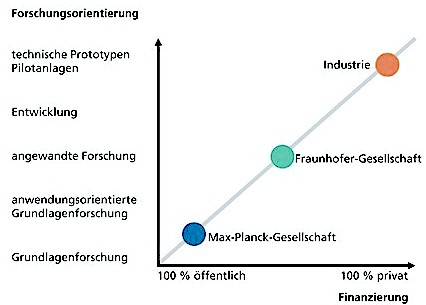
\includegraphics[width=1\textwidth]{pics/finanzenFraunhofer}
      \end{column}
    \end{columns}
  \end{frame}
}

%------------------------------------------------------------------------
\begin{frame}[t] \frametitle{Struktur der Fraunhofer Gesellschaft}
  \begin{columns}
    \onslide<1-2>{
    \begin{column}{0.55\textwidth}
      \begin{itemize}
      \item etwa 22.000 Mitarbeiter, \"uberwiegend Naturwissenschaftler und Ingenieure
      \item dezentrale Organisation durch 
        \begin{itemize}
        \item 66 Fraunhofer-Institute
        \item 10-20 kleinere Forschungseinrichtungen
        \item weitere Niederlassungen au\ss erhalb Deutschlands
        \end{itemize}
      \item Zentrale in M\"unchen
      \item 40 Standorte in Deutschland, darunter auch z.B. SCAI in Sankt-Augustin
      \item die Institute sind in ``Verb\"unden'' zusammengefasst
      \end{itemize}
    \end{column}}
    \begin{column}{0.40\textwidth}
      \invisible<1>{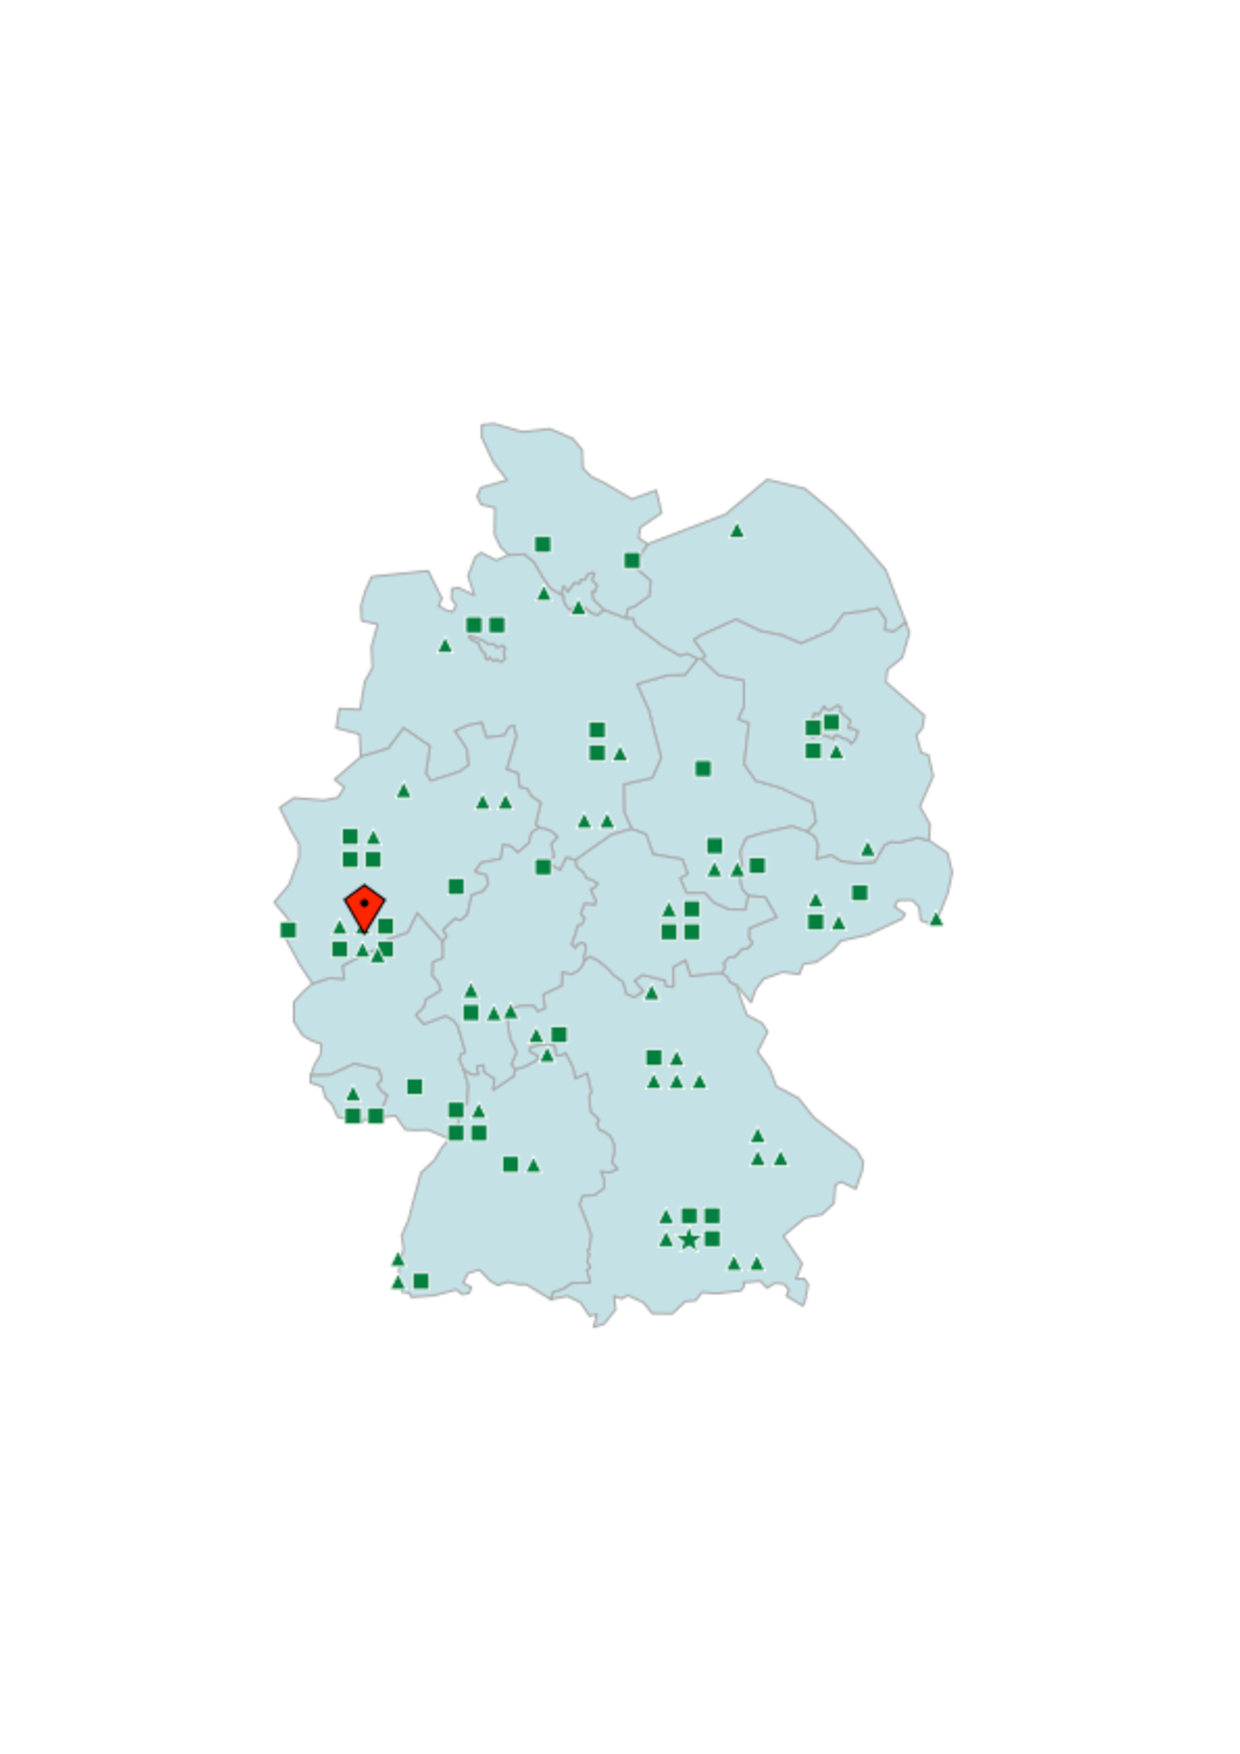
\includegraphics[width=1.0\textwidth]{pics/mapFraunhofer}}
    \end{column}
  \end{columns}
\end{frame}

%------------------------------------------------------------------------


 \section{Das Fraunhofer ESK}
%------------------------------------------------------------------------

\mode<presentation>{
  \begin{frame}[t] \frametitle{\"Uberblick zum Fraunhofer ESK}
    \begin{itemize}
    \item Fraunhofer ESK steht f\"ur {Fraunhofer-Institut f\"ur \textbf{\usebeamercolor[fg]{structure}E}ingebettete \textbf{\usebeamercolor[fg]{structure}S}ysteme und \textbf{\usebeamercolor[fg]{structure}K}ommunikationstechnik}
    \item kleines Institut: ca. 80 feste Mitarbeiter und etwa 20 Studenten
    \item Standort: M\"unchen
    \item Forschungsschwerpunkt: Verfahren und Methoden der Informations- und Kommunikationstechnik (IKT)
    \item Anwendungen u.a. in:
      \begin{itemize}
      \item Fahrzeugkommunikation und Verkehr
      \item Telekommunikation
      \item Sicherheitstechnik
      \end{itemize}
    \item Gliederung in drei Gesch\"aftsfelder:
      \begin{itemize}
        \item {\usebeamercolor[fg]{structure}Automotive}: Fahrzeugkommunikation
        \item {\usebeamercolor[fg]{structure}Industrial communication}: Automatisierung, Kommunikationssysteme f\"ur Energieversorgung
        \item {\usebeamercolor[fg]{structure}Telecommunication}: \"Ubertragungstechniken, Konnektivit\"at von Kommunikationssystemen
      \end{itemize}
    \end{itemize}
  \end{frame}
}

%------------------------------------------------------------------------
\begin{frame}[t] \frametitle{Gesch\"aftsfeld Automotive}
  \begin{columns}
    \begin{column}{0.55\textwidth}
      \begin{itemize}
      \item Gr\"o\ss tes Gesch\"aftsfeld des ESK (etwa 40 Mitarbeiter)
      \item arbeitet an L\"osungen um die wachsenden Anforderungen an Fahrzeuge (Sicherheit, Flexibilit\"at) zu erf\"ullen:
        \begin{itemize}
          \item bessere Vernetzung von Fahrzeugen
          \item Kommuninkationssysteme f\"ur neuartige Fahrzeugkonzepte (bspw. Elektromobilit\"at)
        \end{itemize}
      \end{itemize}
    \end{column}
    \begin{column}{0.4\textwidth}
      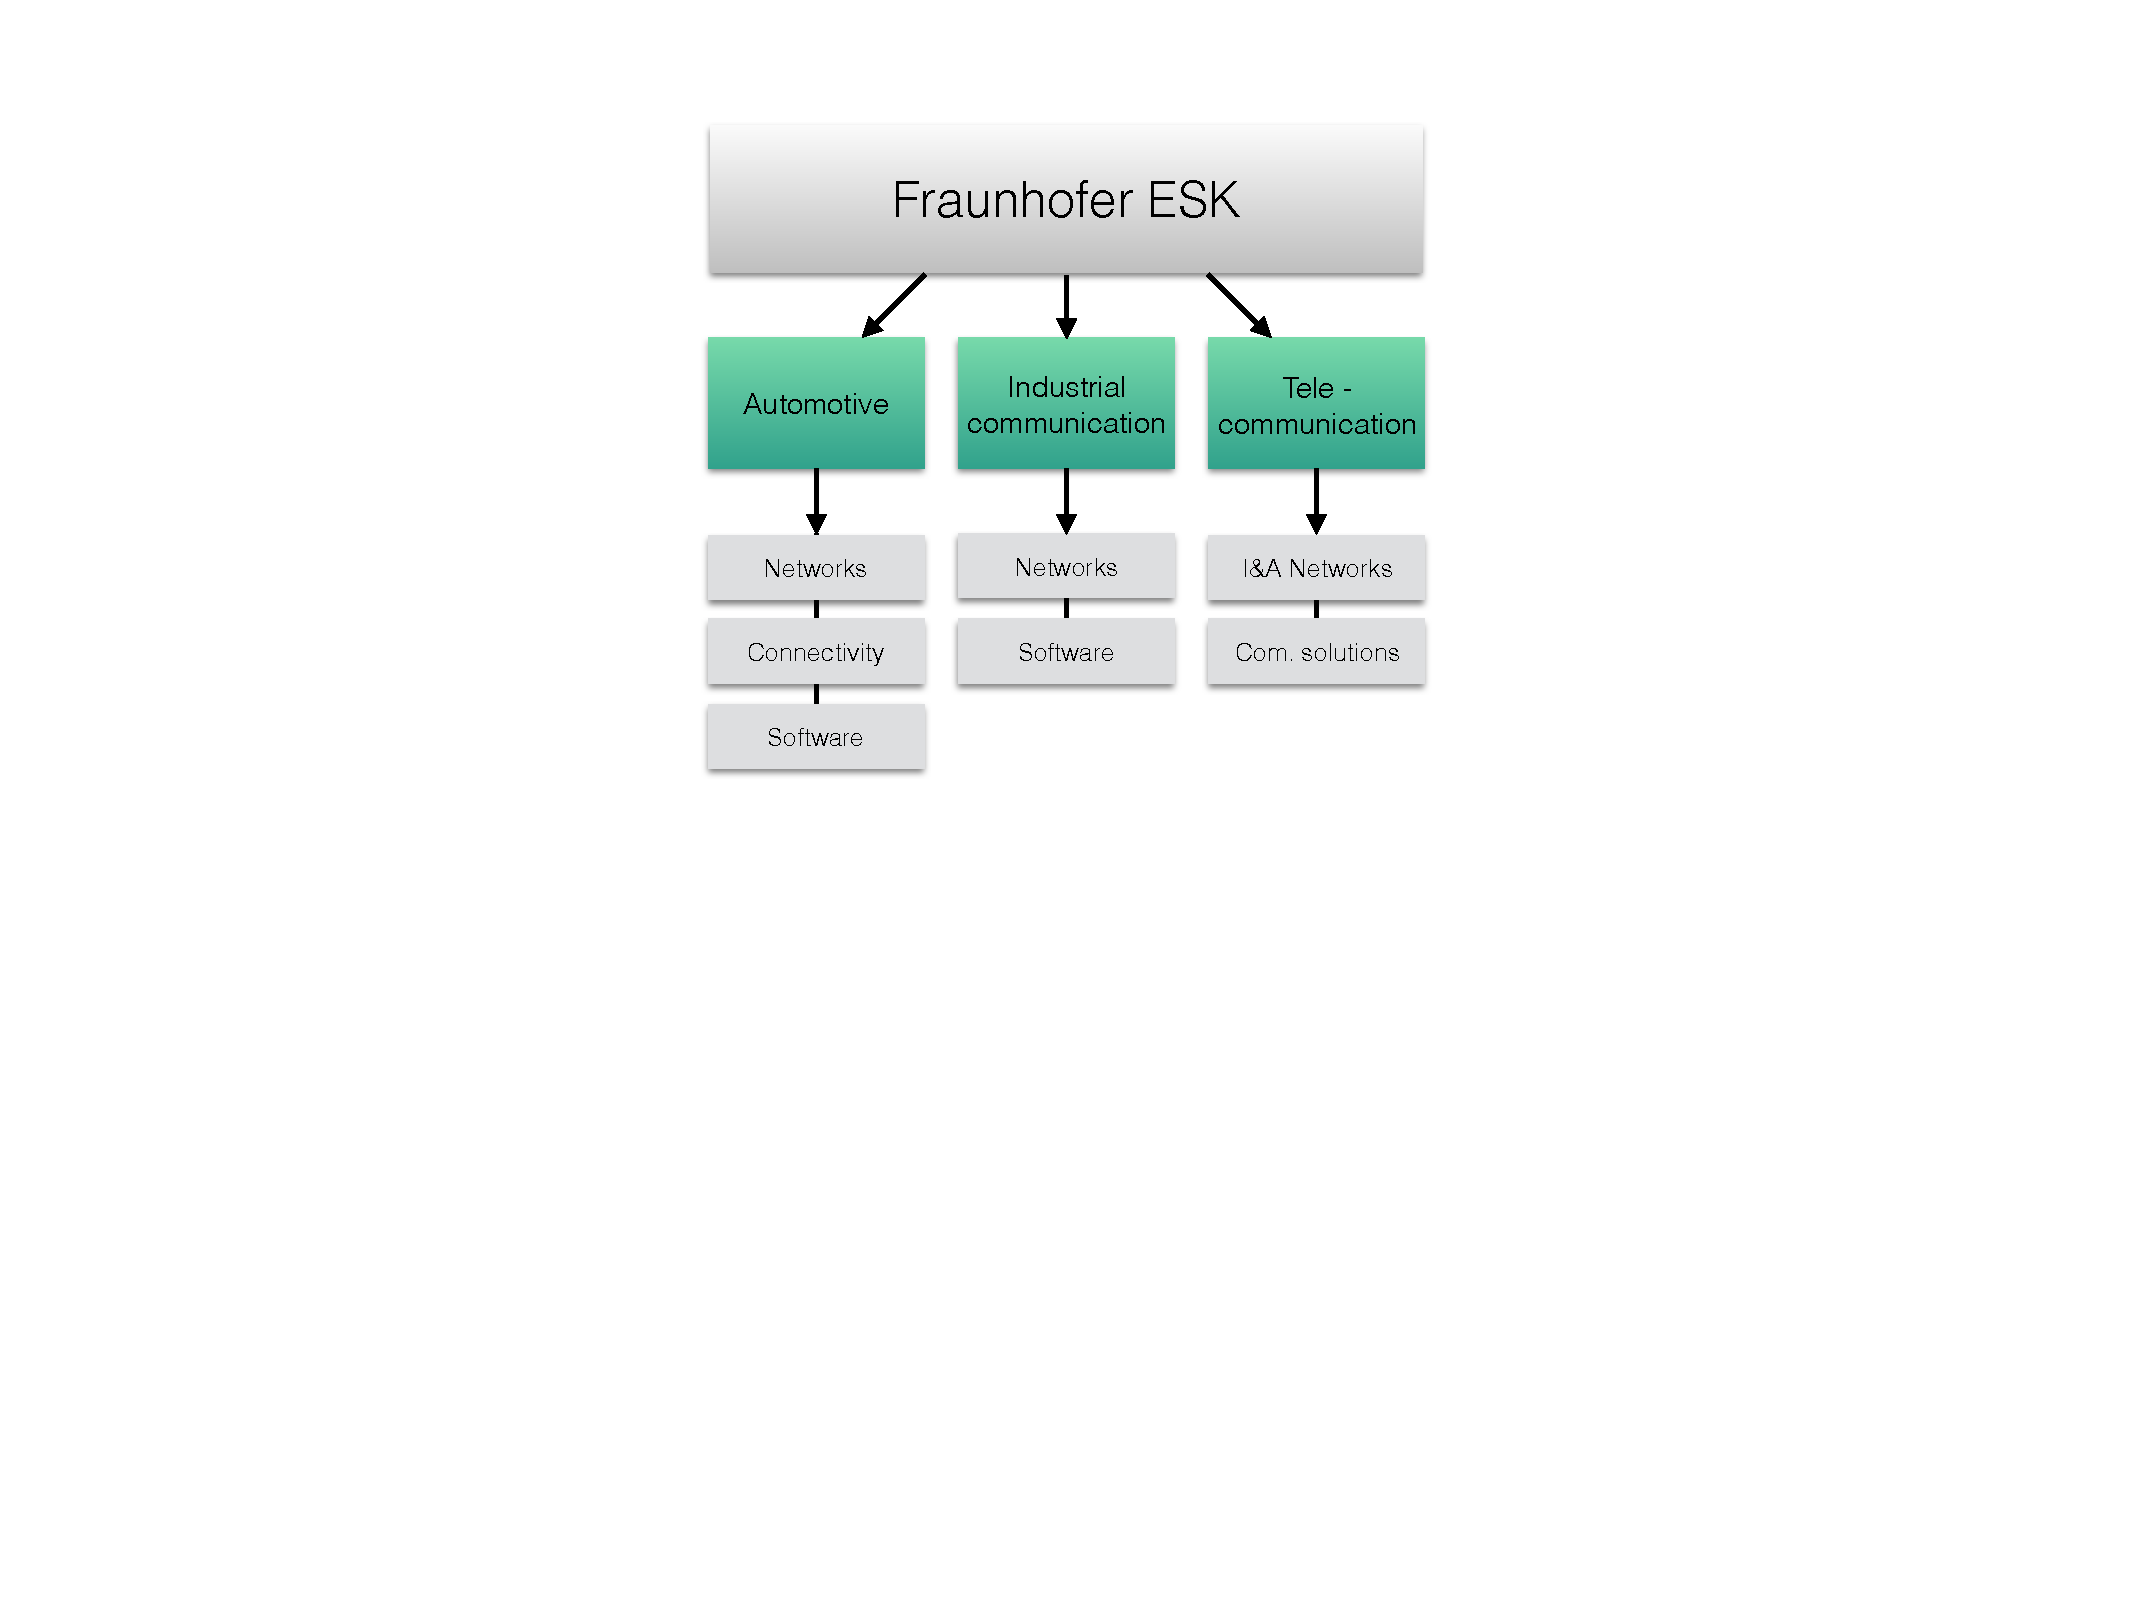
\includegraphics[width=1\textwidth]{pics/chartFraunhofer}
    \end{column}
  \end{columns}
  \begin{itemize}
  \item Automotive Connectivity: Entwicklungen zur Vernetzung von Fahrzeugen untereinander und mit der Umwelt (sog. Car-to-X Kommunikation, kurz C2X) zur Vermeidung von Unf\"allen und Staus
    \begin{itemize}
      \item Datenaggregation und -weiterleitung
      \item Simulationen
      \item Entwicklung von Software-Frameworks
    \end{itemize}
  \end{itemize}
\end{frame}

 \section{T\"atigkeiten w\"ahrend des Praktikums}
\subsection{Organisation und Bewerbung}
%------------------------------------------------------------------------
\mode<presentation>{
  \begin{frame}[t] \frametitle{Organisation und Bewerbung}
    \vspace{0.5cm}
    \begin{itemize}
      \item Praktikumsbeschreibung: Implementierung von kartenbezogenen Algorithmen (in C++)
      \item Zeitraum von ungef\"ahr 5 Monaten
      \item Vollzeit: 39 h/Woche mit bestimmten Kernzeiten
      \item verg\"utet
      \item regelm\"a\ss ige Abstimmung mit Betreuer
        \vspace{0.5cm}
      \item Bewerbungsprozess:
        \begin{itemize}
        \item Bewerbung um ausgeschriebene Praktikumsstelle (\url{https://recruiting.fraunhofer.de/}) %Bewerbung im Zeitraum Mitte-März
        \item Bewerbungsgespr\"ach mit sp\"ateren Betreuer
        \end{itemize}
    \end{itemize}
  \end{frame}
}

\subsection{Aufgabenbeschreibung}
%------------------------------------------------------------------------
\begin{frame}[t] \frametitle{Aufgabenbeschreibung}
  \begin{itemize}
  \item Implementierung von kartebezogenen Algorithmen f\"ur ein Softwareframework im Bereich der C2X-Kommunikation
    \begin{itemize}
    \item {\usebeamercolor[fg]{structure}Routing-Algorithmen:} Bestimmung des ``besten'' Weges zwischen zwei Positionen
    \item {\usebeamercolor[fg]{structure}Mapmatching-Algorithmen:} Abgleich von Kartenmaterial und Standortdaten (GPS-Position)
    \end{itemize}
  \item Implementierung und Test von ausgew\"ahlten Algorithmen
  \end{itemize}
  \begin{columns}
    \begin{column}{0.35\textwidth}
      \begin{itemize}
      \item M\"ogliche Anwendungsf\"alle: 
        \begin{itemize}
        \item \emph{mobincity} (EU-Projekt)
        \item \emph{Adaptive City mobility} (nationales Projekt)
        \item ...
        \end{itemize}
      \end{itemize}
    \end{column}
    \begin{column}{0.6\textwidth}
      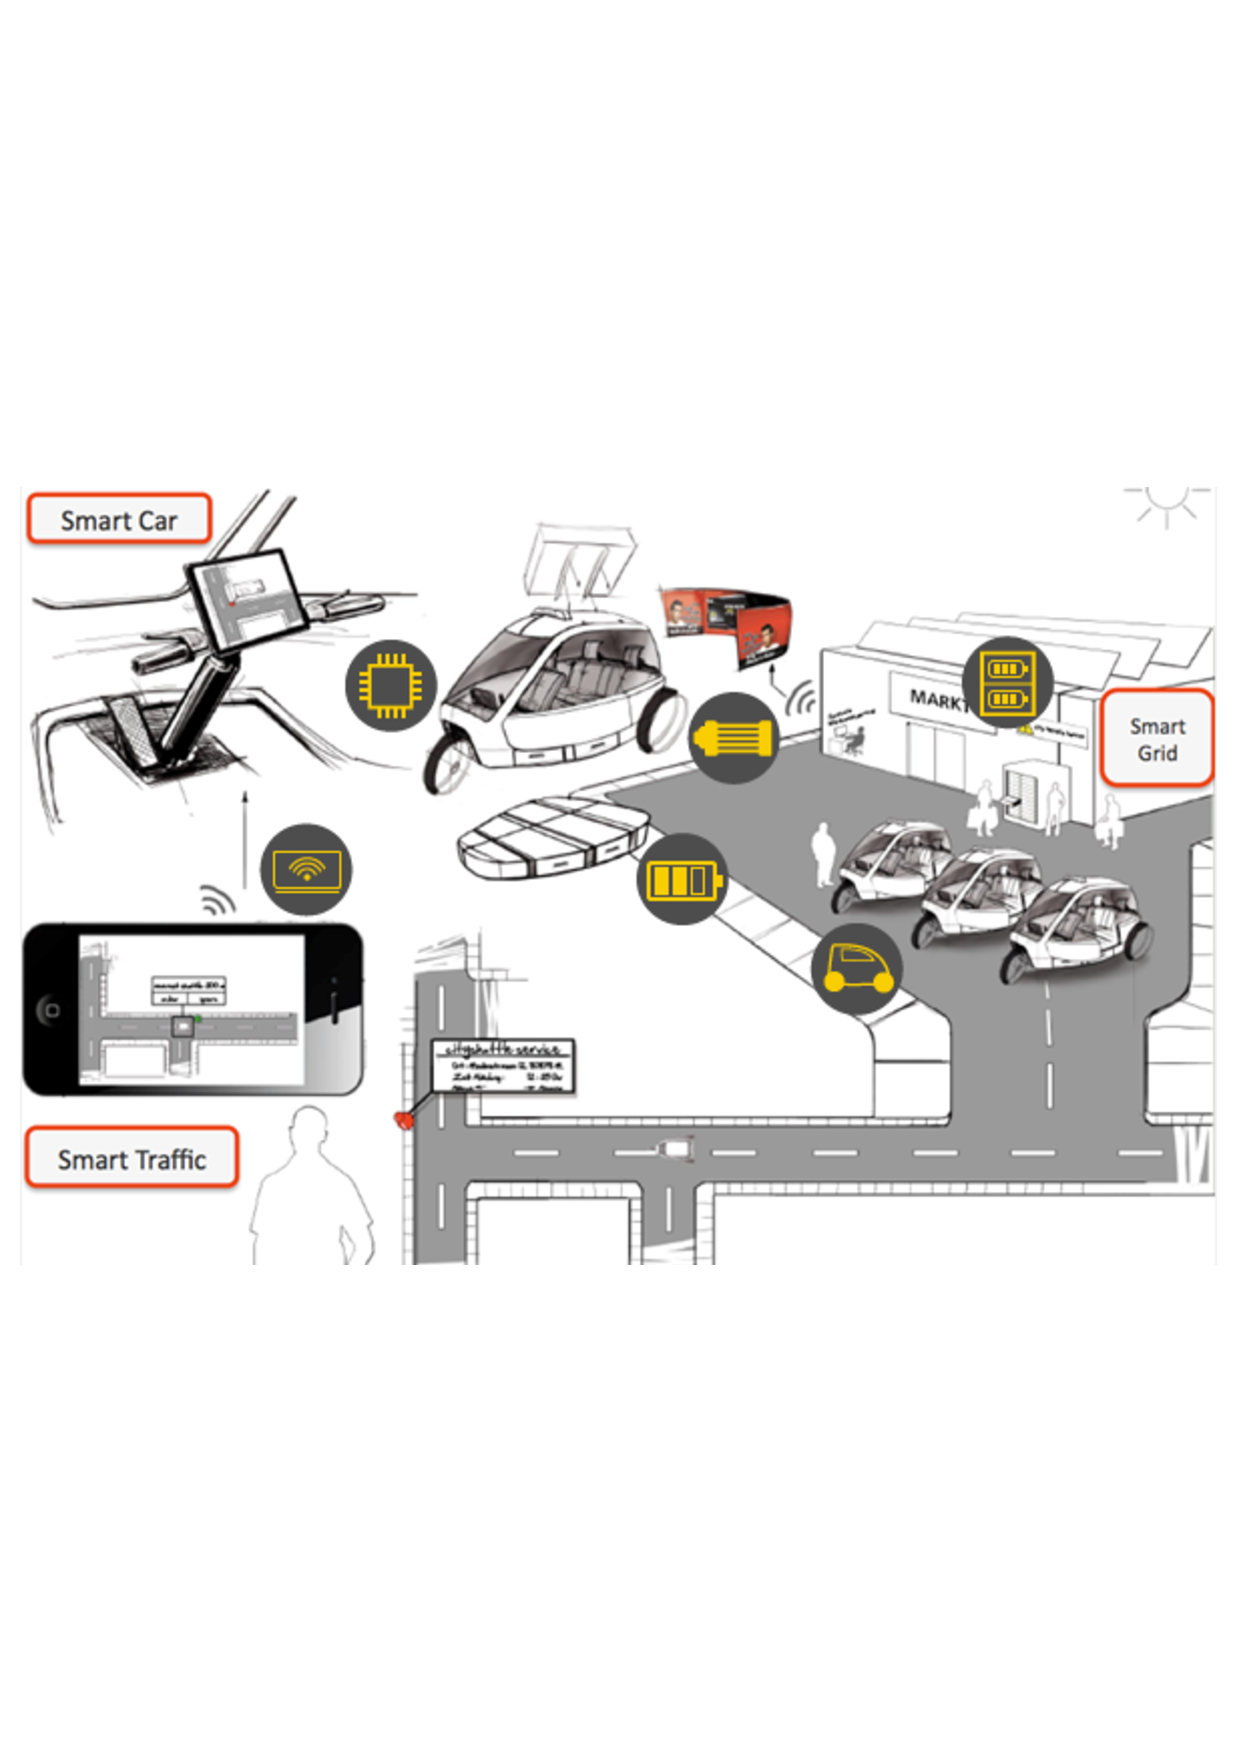
\includegraphics[width=1\textwidth]{pics/acmFraunhofer}
    \end{column}
  \end{columns}
\end{frame}

%------------------------------------------------------------------------
\begin{frame}[t] \frametitle{Arbeitsprozess}
\vspace{0.5cm}
  \begin{itemize}
  \item bereits vorhandenes Framework:
    \begin{itemize}
    \item linzenzkostenfreies Kartenmaterial vom OpenStreetMap-Projekt (osm-Files)
    \item Framework zum Einlesen des Kartenmaterials
    \end{itemize}
  \item Arbeitsprozess:
    \begin{itemize}
    \item Selbstst\"andige Recherche (Internet, Paper)
    \item Entwurf eines Software-Modells
    \item Anpassung und Implementierung
    \item Tests
    \end{itemize}
  \item kleinere Nebent\"atigkeiten
  \end{itemize}
\end{frame}

\subsection{Routing}
%------------------------------------------------------------------------
\begin{frame} \frametitle{Implementierung von Routing-Algorithmen}
  \begin{itemize}
    \item Grundlage: angepasster Dijkstra-Algorithmus
      \begin{itemize}
      \item Abbiegeverbote (Routing \"uber Kanten anstatt Knoten)
      \item Einbahnstra\ss en
      \item Kreisverkehre
      \end{itemize}
      \vspace{0.1cm}
    \item Verbesserung der Laufzeit durch bidirektionale Suche
      \vspace{0.1cm}
    \item Verbesserung des Dijkstra-Algorithmus durch Heuristiken (Sch\"atzfunktionen): Verbesserung der Laufzeit
      \begin{itemize}
      \item euklidische Heuristik: A*-Algorithmus
      \item Landmarken-Heuristik (ben\"otigt Vorberechnung): ALT-Algorithmus
      \end{itemize}
      \vspace{0.1cm}
    \item Kombination von bidirektionaler Suche und Heuristiken
  \end{itemize}
\end{frame}

\begin{frame}[t] \frametitle{Routing-Beispiel}
  \begin{columns}
    \begin{column}{0.3\textwidth}
      \includegraphics<1-3>[width=1\textwidth]{pics/dijkstraFraunhofer}      
    \end{column}
    \begin{column}{0.3\textwidth}
      \includegraphics<2-3>[width=1\textwidth]{pics/biDijkstraFraunhofer}      
    \end{column}
    \begin{column}{0.3\textwidth}
      \includegraphics<3>[width=1\textwidth]{pics/altFraunhofer}      
    \end{column}
  \end{columns}
\end{frame}

\subsection{Mapmatching}
% ------------------------------------------------------------------------
\begin{frame} \frametitle{Implementierung von Mapmatching-Algorithmen}
  \begin{itemize}
  \item einfache geometrische Mapmatching-Algorithmen:
    \begin{itemize}
    \item Matching auf n\"achstgelegenen Knoten
    \item Matching auf n\"achstgelegene Kante (``orthogonale'' Projektion)
    \end{itemize}
  \item topologischer Mapmatching-Algorithmus: berechnet wahrscheinlichste Match-Position durch zus\"atzliche Kriterien:
    \begin{itemize}
    \item Zusammenhang von Stra\ss enabschnitten, Abbiegeverbote
    \item Kurs-Informationen
    \item Geschwindigkeitsdaten
    \end{itemize}
  \item MHT Mapmatching (multiple-hypothesis-technique)
    \begin{itemize}
    \item \"ahnlich zum topologischen Mapmatcher
    \item betrachtet mehrere Kandidaten-Routen gleichzeitig
    \end{itemize}
  \end{itemize}
\end{frame}

\begin{frame}[t] \frametitle{Mapmatching-Beispiele}
  \begin{columns}
    \begin{column}{0.45\textwidth}
      \includegraphics<1-2>[width=1\textwidth]{pics/pointRoadFraunhofer}
    \end{column}
    \begin{column}{0.45\textwidth}
      \includegraphics<2>[width=1\textwidth]{pics/weightTopoFraunhofer}
    \end{column}
  \end{columns}
\end{frame}
 \section{Mathematischer Bezug}
% ** Mathematik im Praktikum

% + *mathematisches Fachwissen ist von Vorteil, aber nicht zwingend notwendig*
%   - *Grundkenntnisse in der Graphentheorie (Dijkstra etc.)*
%   - *Kenntnisse in Geometrie für den Umgang mit dem WGS84 Koordinatensystem*
%   - *Für kompliziertere Mapmatching-Algorithmen: Stochastik (Kalman Filter), Logik (Fuzzy Logic)*
% + *Wichtiger ist "mathematische" Denkweise* /Anmerkung: strukturiertes, logisches Denken/
%   - *organisierte Arbeitsweise*
%   - *unüberschaubare Problemstellungen auf Kernprobleme reduzieren (zum Beispiel: Probleme in Teilprobleme unterteilen)* /Anmerkung: Abstraktionfähigkeit, zum Beispiel geometrischer Mapmatcher/
%   - *Anwenden von abstrakten Theorien auf Probleme der realen Welt (zum Beispiel: Berücksichtigung von Abbiegeverboten im Dijkstra-Algorithmus)* /Aufgabenlösen im Studium/
% + *Schnelle und selbständige Einarbeitung in neue Themenbereiche* /Im Mathematikstudium durch Seminare/
%   - *Verständnis und Bewertung von neuen Algorithmen*
%   - *Zurechtfinden in neuen Datenstrukturen* /Anmerkung: großes Software repository, Software Bibliotheken/
% + *Hohe Frustrationstoleranz*
% + *Gute Fähigkeiten am Computer* /Anmerkung: ist nicht wirklich Mathematik-Typisch, aber Programmieraufgaben sind gut.../

%------------------------------------------------------------------------
\mode<presentation>{
  \begin{frame}[t] \frametitle{Mathematischer Bezug im Praktikum}
    \vspace{0.5cm}
    \begin{itemize}
    \item mathematisches Fachwissen ist von Vorteil, aber nicht zwingend
      \begin{itemize}
      \item Grundkenntnisse der diskreten Mathematik (Graphentheorie, Dijkstra-Algorithmus)
      \item Geometrie f\"ur Distanz-Berechnung auf gekr\"ummten Fl\"achen
      \item Stochastik (Kalman Filter), Logik (Fuzzy Logic) f\"ur kompliziertere Mapmatching-Algorithmen
      \end{itemize}
      \vspace{0.5cm}
    \item Wichtig: \emph{``mathematische''} Denkweise
      \begin{itemize}
      \item Reduktion auf Kernprobleme bei un\"uberschaubaren Problemstellungen (z.Bsp. Probleme in Teilprobleme unterteilen)
      \item Anwenden von abstrakten Theorien auf Probleme der realen Welt (z. Bsp. Ber\"ucksichtigung von Abbiegeverboten im Dijkstra-Algorithmus)
      \end{itemize}
    \end{itemize}
  \end{frame}  
}

%------------------------------------------------------------------------

\begin{frame}[t] \frametitle{Mathematischer Bezug im Praktikum}
  \vspace{1cm}
  \begin{itemize}
  \item Eingenst\"andiges und schnelles Einarbeiten in neue Themenbereiche
    \begin{itemize}
    \item Verst\"andnis und Bewertung von neuen Algorithmen
    \item Zurechtfinden in neue Datenstrukturen
    \end{itemize}
  \end{itemize}
\end{frame}

%------------------------------------------------------------------------

 \section{Pers\"onliches Fazit und Ausblick}
%------------------------------------------------------------------------
\mode<presentation>{
  \begin{frame}[t] \frametitle{Pers\"onliches Fazit}
    \begin{description}
    \item[Insgesamt]
      \begin{itemize}
      \item sehr positive Erfahrung
      \item guter Einblick in die Arbeit in einer Forschungsorganisation 
      \end{itemize}
    \item[Pro] 
      \begin{itemize}
      \item angenehme Arbeitsatmosph\"are
      \item weitesgehend selbstst\"andiges Arbeiten mit vielen eigene Entscheidungen
      \item interessantes und abwechslungsreiches Themengebiet
      \item Motivation durch schnell erkennbaren Fortschritt
      \end{itemize}
    \item[Contra]
      \begin{itemize}
      \item wenig Einblicke in andere Bereiche des Instituts
      \item zu wenig Zeit, um interessantere Algorithmen zu implementieren
      \item keine M\"oglichkeit eigene Ideen f\"ur Algorithmen umzusetzen
      \end{itemize}
    \end{description}
  \end{frame}  
}

%------------------------------------------------------------------------
\begin{frame} \frametitle{Ausblick}
  \begin{itemize}
  \item gro\ss e Hilfe bei der Orientierung f\"ur einen sp\"ateren Beruf
    \begin{itemize}
    \item mathematisches Fachwissen ist nicht alles
    \item kompetenter Umgang mit Computern ist von Vorteil
    \end{itemize}
  \item erm\"oglicht bessere Ausrichtung des Studiums
  \item sp\"atere Anstellung bei der Fraunhofer Gesellschaft vorstellbar
    \begin{itemize}
    \item m\"oglicherweise andere Bereich (z.Bsp. mit physikalischen Hintergrund)
    \item evtl. w\"ahrend einer m\"oglichen Promotion
    \end{itemize}
  \end{itemize}
\end{frame}

%------------------------------------------------------------------------
\begin{frame} \frametitle{Kontakte}
  \begin{description}
  \item[Meine Email-Adresse: \hspace{2cm}] 
    \url{pascal.huber@uni-bonn.de}
  \item[Stellenangebote der Fraunhofer-Gesellschaft] \url{https://recruiting.fraunhofer.de}
  \end{description}
\end{frame}

\begin{frame}[c]
  \begin{center}
    \huge{\usebeamercolor[fg]{structure}Vielen Dank f\"ur eure Aufmerksamkeit!} \\
    \vspace{1cm}
    \large{\usebeamercolor[fg]{structure}(Fragen?)}
  \end{center}
\end{frame}

\section{Quellen}
%------------------------------------------------------------------------
\begin{frame} \frametitle{Quellen}
  \begin{description}
  \item[Homepage der Fraunhofer Gesellschaft] \url{http://www.fraunhofer.de}
  \item[Homepage des Fraunhofer ESK] \url{http://www.esk.fraunhofer.de}
  \item[Projekte mit C2X-Anwendung] 
    \url{http://www.adaptive-city-mobility.de} 
    \url{http://www.mobincity.eu}
  \item[Seite des OpenStreetMap-Projekts] \url{http://www.openstreetmap.org/}
  \end{description}
\end{frame}


\end{document}

 